\chapter{Plagiarism in Modeling Assignments}\label{cha:mde1}


As modeling assignments become more common in computer science education~\cite{Ciccozzi2018, Brambilla2017}, plagiarism detection for these assignments becomes more relevant. However, there is little research on plagiarism detection for artifacts of modeling assignments \cite{Martinez2020}.
This chapter discusses the challenges of modeling plagiarism, presents a controlled experiment on how novice modelers obfuscate plagiarism, and empirically explores how generative AI can be exploited for modeling plagiarism.
This chapter discusses the nuances of plagiarism within modeling assignments, including obfuscation techniques and effective detection methods.

The remainder of the chapter is structured as follows:
First, in \autoref{sec:mde-considerations}, we examine the differences between modeling artifacts and code. We outline four key challenges that arise when detecting plagiarism in modeling contexts.
One of these challenges, the lack of knowledge on modeling plagiarism, is explored in \autoref{sec:human-plagiarism} through an experiment investigating how novice modelers engage in plagiarism.
Finally, \autoref{sec:ai-plagiarism} explores the automated aspect of obfuscation, examining how generative AI can be exploited to facilitate plagiarism in modeling assignments.

\ownpublications{
    \fancycite{Saglam2024a},
    \fancycite{Saglam2023}, and
    \fancycite{Kienzle2024}.
}

%\section{Challenges of Modeling Plagiarism}
\section{Understanding Modeling Plagiarism}\label{sec:mde-considerations}

\noindent
In traditional software engineering, code represents instructions for a computer program's behavior, while models represent abstract concepts and relationships between entities in a system.
This distinction is, however, blurred, as code can be considered just another model in the context of model-driven engineering~\cite{Stachowiak1973}. This aligns with the mantra \enquote{\textit{everything is a model}} \cite{Bezevin2005}. Code can be viewed as a lower-level model, which is often derived from higher-level, abstract models. Both models and code are interconnected representations of the same system, with code being an executable model that conforms to the specifications of higher-level models.
Most modeling artifacts have graph-like or tree-like structures or can be transferred into them, for example, through containment references in \ac{MOF}-based metamodels.
Similarly, while code is a text-based entity, it can be parsed into a parse tree, for example, an \ac{AST}.
Thus, models can, just like code, describe a program's structure and behavior. However, in practice, there are differences between \textit{typical} modeling assignments~\cite{Ciccozzi2018} and typical programming assignments~\cite{Schulte2006}.

%\subsection{Assumptions}
Based on the mentioned differences, we make the following assumptions.
Modeling assignments often focus on creating high-level abstractions, such as diagrams and formal specifications, which capture the structure, behavior, and relationships of a system. These assignments emphasize understanding and representing domain concepts accurately and may involve tools and languages specific to modeling, such as \ac{UML}, \ac{EMF} or \ac{SysML}~\cite{Kienzle2024}. On the other hand, programming assignments typically require students to write executable code that directly implements algorithms and functionality. These assignments emphasize problem-solving, algorithmic thinking, object-oriented modeling, and mastery of programming language syntax.
As a result, the skills and tasks involved in modeling assignments differ from those in programming assignments. 
Based on these assumptions, notable differences exist between models and code in the context of plagiarism detection.

\subsection{Requirements for Detection Systems}
Based on these differences, we identify the following requirements for modeling plagiarism detection:
% Basic Requirements:
Modeling assignments pose a unique challenge because models typically operate at a higher level of abstraction, providing fewer details for detection~\cite{Saglam2022}. Furthermore, approaches designed for code rely on linearization, a process that is not trivial for models in general~\cite{Saglam2024a}. 
Last, visualization of suspicious candidates necessitates specialized graphical or textual views to provide the necessary explainability~\cite{Karnalim2021} for effective plagiarism detection. For code, this is trivial, as the code itself can be used~\cite{Saglam2024a}.

Consequently, there is a need for a tool-based solution that addresses these challenges and tackles the problem at scale~\cite{Saglam2023}.
Such a solution must provide explainability and traceability for educators to understand why a student submission is identified as suspicious.
Thus, a good plagiarism detector informs and assists educators in decision-making and processes in misconduct investigations, which vary significantly across institutions.
Tool-based solutions should help educators by identifying suspicious candidates while leaving final decision-making to the educators to uphold ethical standards~\cite{Le2013}.

% Key Requirement: Compatibility with different modeling languages
Another crucial aspect is modeling language compatibility, which allows educators to benefit widely from these approaches.
Educators may find the use of plagiarism detectors infeasible if a significant effort is required to tune plagiarism detectors for specific modeling languages or artifacts; using them becomes infeasible.
Generalized approaches independent of specific modeling languages or tools are not intricate enough to provide helpful feedback for any modeling assignment.
%

Educators must be conscious of these limitations. Therefore, plagiarism detectors should be designed to enable educators to recognize situations where the results lack conclusiveness, enabling them to make well-informed and ethical decisions.
In the following, we will discuss four differences between modeling artifacts and code that present challenges for (token-based) plagiarism detection of modeling artifacts.

\subsection{Challenges}\label{sec:mde-challenges}
We identify the need for effective plagiarism detection approaches for modeling artifacts that are mature enough for practical application. There is significant interest in this topic among educators in the model-driven community, especially with the recent rise of generative AI\footnote{This interest led to my invitation to deliver a keynote~\cite{Saglam2024Keynote} at the \textit{Educators Symposium} of the 2024 \textit{MODELS} conference~\cite{models2024_preface}.}.
However, modeling plagiarism detection comes with the following \textbf{challenges}:
\paragraph{Abstraction Level and Granularity}
Modeling artifacts typically represent a system at a higher level of abstraction than code, thus often containing less detail, which presents an added challenge for plagiarism detection~\cite{Saglam2022}.
Moreover, the granularity of modeling artifacts can vary significantly. Modeling artifacts can range from high-level conceptual models to detailed design specifications. These models often capture domain concepts and relationships at a higher level of abstraction, which may not directly map to concrete implementations. In contrast, code is generally more consistent in granularity, focusing on implementation details. Code is directly executable and is closer to the machine level, with precise operational semantics. This means that code typically includes more details than modeling artifacts, making distinguishing between unrelated similarities and actual plagiarism easier. However, in modeling assignments, the lack of details can make it harder to identify plagiarism, as superficial similarities may be more common and less indicative of copying~\cite{Saglam2024a}.
It is an inherent challenge in plagiarism detection that in small assignments, the solution space collapses, rendering it impossible to differentiate between plagiarism and random, disjointed similarities.
This problem, while present in coding assignments with a small solution space, is exacerbated for modeling assignments due to the higher level of abstraction and varying granularity.

\paragraph{Structural Complexity}
Modeling artifacts often involve complex, hierarchical structures such as metamodels, models, and transformations. These can also include behavioral models, which add another layer of complexity. For example, a behavioral model might describe the dynamic behavior of a system through state machines or sequence diagrams. In contrast, code is \textit{typically} linear and sequential, with a linear declaration order via statement order and a primarily linear execution order, as code defines partial order for statement interdependence, making it easier to tokenize and linearize. Although there are some exceptions, this generally holds true for programming languages commonly used in education and for most language constructs within their syntax.
The sequence of statements in code is critical in determining the code's behavior. While some statements can be reordered without changing the code's behavior, there is only a limited possibility of doing so.
Therefore, the reordering of statements must be executed with caution, as it can drastically modify the program's functionality.

In contrast, the degree to which the order of elements in a model affects the system behavior depends on the metamodel and the model's intended use. Often, the order of elements in a model, especially in multi-valued containment references, can be freely altered. Even if it cannot be freely changed, some degrees of freedom usually exist.
Moreover, the structural aspects of modeling artifacts mean that strategies for tokenization and comparison can vary significantly between different types of models. Behavioral models, in particular, present a challenge due to their dynamic nature and the need to capture semantic aspects and interactions, which are less straightforward to represent and compare in a linear token-based approach.

\paragraph{Representation and Notation}
Modeling artifacts use diverse notations, often graphical, such as \ac{UML} diagrams. These notations may not be easily linearizable (or at least not in a meaningful manner), and their serialized representation in files is often not human-readable or directly representative of their semantic or graphical form~\cite{Harel2004}. In contrast, code uses textual syntax with well-defined semantics, and the representation in files is also the representation used by humans. This difference means that visualizing matched subsequences for plagiarism detection cannot be done effectively using the file representation alone for modeling artifacts. Instead, a specific view tailored to the type of modeling artifact is required to accurately represent and compare the structures and relationships captured in the model.

\paragraph{Models and Semantics}
In the context of model-driven engineering, there is no universal definition of semantics for models.
Unlike code, models are often not executable. For metamodels, we typically distinguish static semantics from dynamic semantics~\cite{Stahl2006}. The static semantics describe rules and constraints that are not expressed through the abstract syntax. The dynamic semantics express the meaning of the constructs. Dynamic semantics is often specified not formally but only through natural language text~\cite{Brambilla2017}.
As a consequence, the differentiation between semantic-preserving, semantic-agnostic, and semantic-deviating obfuscation is blurred in the context of modeling plagiarism. Only if there is a clearly defined dynamic semantics, for example, for executable models, can this separation be made to the same extent as for code.

\paragraph{Obfuscation Techniques}
As students tend to be creative in obfuscating their plagiarism~\cite{Saglam2023, Karnalim2016}, plagiarism detectors must be resilient against common obfuscation attempts.
The techniques for obfuscating modeling artifacts are less clear than those for code. Most research on plagiarism detection focuses on code~\cite{prechelt2000, MOSS, Maertens2022}, where common obfuscation techniques are well researched~\cite{Faidhi1987, Karnalim2016, Novak2019, Novak2020}. There is substantial research on code obfuscation and its impact on plagiarism detection. However, the lack of extensive research on how modeling artifacts are obfuscated presents a challenge for token-based plagiarism detection in this domain. The unknown nature of potential obfuscation techniques for models makes it difficult to develop robust defense methods.


\section{Manual Obfuscation in Modeling Assignments}\label{sec:human-plagiarism}
% --------------------------
% Related Work / Gap
% --------------------------
How students plagiarize programming assignments and which ways they employ to obfuscate their plagiarism is well researched \cite{Novak2019}.
This includes classifications of code obfuscation techniques \cite{Faidhi1987, Karnalim2016} and the automated detection of plagiarism in student submissions \cite{prechelt2002}.
However, as discussed in \autoref{sec:mde-challenges}, only limited research exists on plagiarism in modeling assignments. Furthermore, modeling assignments are susceptible to plagiarism since they are complex and require domain understanding and problem-solving skills \cite{Martinez2020}.
Yet, these assignments are often the only way to evaluate the student's performance~\cite{Ciccozzi2018}.
How students engage in plagiaristic behaviors in modeling assignments remains unclear.
Related work from the domain of modeling clone detection \cite{Babur2019} does not address this issue: Plagiarism detection involves an attacker scenario, where the plagiarizer intentionally tries to conceal the plagiarism by employing various obfuscation techniques. In contrast, clone detection focuses on identifying identical or similar sections in models without considering deliberate obfuscation by plagiarizers.
Therefore, the insights from modeling clone detection cannot be directly applied to the context of modeling plagiarism.
In essence, the lack of knowledge about students' plagiaristic behaviors hinders detection efforts.

% --------------------------
% Contribution
% --------------------------
We address this gap by systematically analyzing how students plagiarize and obfuscate in modeling assignments.
We present the results of an experiment where ten novice modelers were asked to plagiarize a given metamodeling assignment's solution and conceal their plagiarism, i.e., hiding the relation to the original.
The experiment was conducted in a master-level practical modeling course, where each student was given 30 minutes to conceal the plagiarism in their solution copy.
We employed a mixed-method approach, combining quantitative analysis of the plagiarized metamodels and qualitative data from the participants' descriptions of how they tried to conceal the plagiarism.
We show how frequently different techniques were employed and to what level the models were altered.
In the experiment's result evaluation, we asked the course instructors to inspect both plagiarized and original solutions.
Additionally, we applied a state-of-the-art plagiarism detector~\cite{Saglam2022} to test the automatic plagiarism detection quality.
With this experiment, we set out to answer the following key questions:

\begin{enumerate}%[style=unboxed,leftmargin=0cm,topsep=3pt]
    \item How do novice modelers conceal modeling plagiarism?
    \item Can their modeling plagiarism be detected by the instructors?
    \item Can their modeling plagiarism be detected by plagiarism detectors?
\end{enumerate}

\noindent
The experiment shows how the ten participants engage in modeling plagiarism and how they describe their approach.
%
The results show that the participants employ various obfuscation techniques, with the renaming of elements occurring most frequently, followed by reordering elements.
On average, students alter every second element of the modeling assignment. Nevertheless, human and tool-based inspection can still detect these instances of plagiarism.
However, manual inspection quickly becomes impractical with large course sizes.
This paper contributes to a better understanding of plagiarism in modeling assignments by investigating students' obfuscation techniques.
Ultimately, we provide insights to enhance fairness and academic integrity in assessing modeling assignments.

\subsection{Experiment Design}\label{sec:human-plagiarism-task}
%\todo{slide figure about the process: original --> student --> plag + descr}

\noindent
We conducted an experiment with novice modelers, where they plagiarized an \ac{EMF} metamodel and obfuscated the relation to the original metamodel.
In total, ten students voluntarily participated in the experiment.
%
The experiment consisted of two tasks conducted sequentially.
First, the participants were asked to copy and modify a given source metamodel to conceal the plagiarism while still fulfilling the given assignment.
Second, we asked the participants for a brief description outlining their techniques to disguise the act of plagiarism and its relation to the original solution.
%
We employed a mixed-method approach, combining quantitative analysis of the plagiarized metamodels and qualitative data from the participants' descriptions of how they tried to conceal the plagiarism. 
%
The duration of the experiment was 30 minutes. 
Since participants used their own solutions as a basis for plagiarism, they did not require additional familiarization with the solution. For an experiment where the participants are unfamiliar with the given solution, a larger time frame would have been required.

\textbf{Scenario:}
We instructed the participants to imagine a scenario where a deadline for a modeling assignment was coming up. However, they had access to a solution provided by a hypothetical classmate and thus decided to plagiarize it. To that end, the participants were asked to conceal the plagiarism from the instructor of the hypothetical course while still fulfilling the assignment.
In detail, we gave the following instructions regarding the obfuscation:

\begin{myquote}
\textit{1. Create a copy of the metamodel.}
    
\textit{2. Modify the copy to disguise the plagiarism (the examiner will only assess the metamodel).}
    
\textit{3. Make sure that the modifications have been saved.}
\end{myquote}

Finally, we asked them to describe how they proceeded during the task and what types of modifications they used.

\textbf{Participants:}
We conducted our experiment with ten students from a practical course on model-driven software development.
It is a master's level computer science elective course at Karlsruhe Institute of Technology, Germany. 
The students are novice practitioners of model-driven engineering and had little to no prior metamodeling experience before attending the course. They have basic knowledge of \ac{UML} diagrams and object-oriented modeling.
The course covers typical~\cite{Ciccozzi2018} topics like (meta)modeling and model transformations.
They participated in the experiment after completing the course's metamodeling assignment.

\textbf{Metamodeling Assignment:}
Our experiment uses a typical~\cite{Ciccozzi2018} modeling assignment~\cite{Saglam2023_supp} of an \ac{MDE} practical course (master's level elective course, no prior metamodeling experience), which tasks the students with creating an \ac{EMF} metamodel for designing component-based system architectures. The metamodel includes four different architectural views: The component repository, the component assembly, the system's hardware environment, and the components' allocation.
The task is loosely inspired by the Palladio component model~(PCM)~\cite{reussner2016a}.
%
The \textit{repository} manages all components and interfaces that may be reused within multiple systems. The \textit{assembly} shows how components are instantiated and interconnected. The \textit{environment} depicts all containers and their links. The \textit{allocation} specifies which components are allocated on which containers of the environment.
%
The goal of the assignment is to design an \ac{EMF} metamodel that allows modeling systems such as the media store architecture in \autoref{fig:mediastore}.
%
Students usually solve this modeling assignment in groups, ranging between two and five students. 
In the past, students' solutions for this assignment contained, on average, five packages, 39 classifiers, 45 references, ten attributes, and one operation \cite{Saglam2022}.
Most metamodels were designed in a single file, but some students fragmented them into up to 7 files.

\begin{figure}
    \centering
    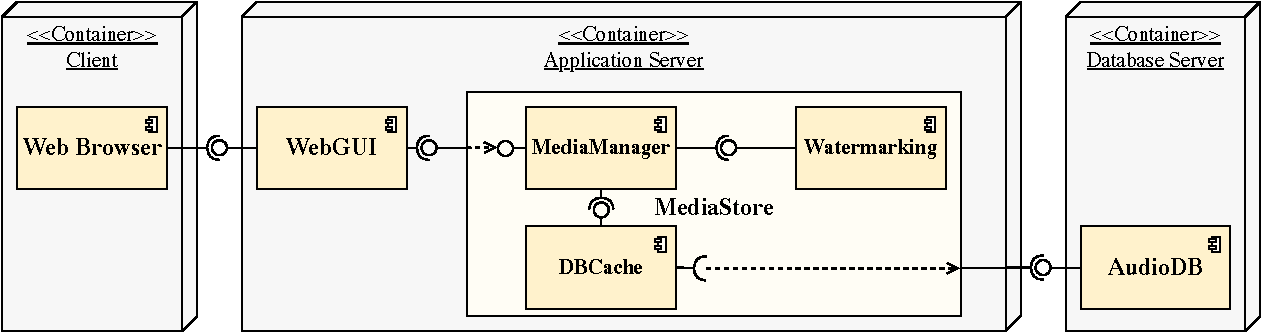
\includegraphics[width=0.99\linewidth]{figures/mediastore.pdf}
    \caption[Example Instance for the Modeling Assignment]{Component-based architecture of a media store, which the assignment's metamodel should be able to represent. Loosely based on the work of \citet{becker2008a}.}
    \label{fig:mediastore}
\end{figure} 

\textbf{Ethical Considerations:}
During this experiment, ethical considerations were given due attention. Participants voluntarily partook and were fully informed about the experiment's scope and purpose. They explicitly agreed to use and publish their artifacts for research purposes, ensuring confidentiality by anonymizing them.% Transparency and respect for participants were principles upheld during the study.

\subsection{Observed Results}
%\todo{(LOW) Examples aus Vortrag zu Figures machen.}


%\citet{Babur2019}:
%\begin{description}[style=unboxed,leftmargin=5pt]
%    \item[Type-A] Exact duplicates except for layout, formatting, internal ids, and cosmetic name changes (lower-/uppercase)
%    \item[Type-B] Duplicates with smaller syntactic/semantic changes to names, types, attributes, and minor additions/removals.
%    \item[Type-C] Duplicate larger changes/additions/removals of elements, names, types, and attributes.
%    \item[Type-D] Semantically duplicates with different structures and content.
%\end{description}

%\citet{Faidhi1987,Karnalim2016}:
%\begin{description}[style=unboxed,leftmargin=5pt]
%    \item[Level 0:] Verbatim copy.
%    \item[Level 1:] Changes in comments and indentation.
%    \item[Level 2:] Changes in names.
%    \item[Level 2.5:] Changes to packages and package namespaces (introduced by \cite{Karnalim2016}).
%    \item[Level 3:] Changes in declarations (e.g., adding extra constants, changing the positions of declared variables, shuffling the methods, etc.).
%    \item[Level 4:] Changes in pro wordgram modules (e.g., encapsulating statements in methods, using either parameters or global variables, inserting dummy methods).
%    \item[Level 5:] Changes in program statements (e.g., using FOR instead of WHILE, etc.).
%    \item[Level 6:] Changes in the decision logic (e.g., changes in expressions, loops to recursion, rearranging loosely coupled statements).
%\end{description}

\begin{table*}[t]
	\centering
    \small
	\begin{tabular}{l p{215pt} r r r} % nach letztem c @{\hskip 2em}
		\toprule
		Techniques         & Description                                                                       & \footnotesize\#Occ. & \footnotesize\#Part. & \footnotesize Type\\
		\midrule
		Cosmetic Renaming  & Changing capitalization of names, introducing or resolving typographical errors.                 & 1    & 1    & A                     \\
		Minor Renaming     & Introducing or resolving abbreviations, adding and removing suffixes or prefixes. & 85   & 9    & B                     \\
		Major Renaming     & Changing names to synonyms, translations, or entirely different names.            & 141  & 7    & C                     \\
		\midrule
		Reorder Features  & Re-ordering attributes and references of a classifier.                            & 10   & 1    & B                     \\
		Reorder Package   & Re-ordering the model elements contained within a single package.                       & 57   & 4    & B                     \\
		Reorder Classifiers & Moving classifiers from one package to another (re-ordering across the model).  & 1    & 1    & C                     \\
		\midrule
		Introduce Package  & Create a package and add existing elements from other packages or other packages. & 20   & 3    & C                     \\
		Dissolve Package   & Deleting a package and moving its contained elements to other packages.           & 8    & 4    & C                     \\
		\midrule
		Delete Feature     & Delete an existing attribute, relation, or operation of a classifier.             & 26   & 7    & B                     \\
		Delete Classifier  & Delete an existing classifier from the model.                                     & 11   & 6    & C                     \\
		Delete Package     & Delete an existing package from the model (can be part of dissolving a package).  & 5    & 4    & B                     \\
		\midrule
        Insert Feature     & Insert a new attribute, relation, or operation into a classifier.                 & 6    & 4    & B                     \\
		Insert Classifier  & Insert a new classifier into the model.                                           & 10   & 3    & C                     \\
		Insert Package     & Inserting a new package into the model (may be combined with moving elements).    & 5    & 4    & B                     \\
		\midrule
        Change Property    & Changing an element's property, e.g., \textit{abstract} for classifiers, \textit{ordered} or the cardinality for references. & 31    & 3    & B                     \\
		\midrule
		Remove Inheritance & Remove inheritance relation between the two classifiers.                          & 4    & 1    & C                     \\
        Add Inheritance    & Add inheritance relation between the two classifiers.                             & 7    & 2    & C                     \\
		Change Inheritance & Changing the inheritance hierarchy structurally without changing it semantically. & 9    & 2    & D                     \\
		\bottomrule
	\end{tabular}
    \caption[Obfuscation Techniques by Novice Modelers]{Overview of the obfuscation techniques employed by the participants, classified according to \citet{Babur2019}. We include how often each technique occurred across all participants (denoted as \textit{\#Occ}) and how many participants employed it (denoted as \textit{\#Part}).}
	\label{tab:student-obfuscation}
%\todo{Do we want the midrules? And if yes how to we want to separate? e.g. for property?}
\end{table*}



\noindent
%
In this section, we present our findings~\cite{Saglam2023_supp}, analyze the participants' obfuscation techniques, examine human plagiarism detection effectiveness, and evaluate an automated tool's detection performance.

\paragraph{Obfuscation Techniques}
To analyze the obfuscation techniques employed by the students, we first used \textit{EMF Compare} to identify potential differences between the plagiarized models and their originals. Unsurprisingly, in some cases, EMF Compare did not accurately produce the correct differences~\cite{Wittler2023}, highlighting the limitation of relying solely on model differencing for plagiarism detection.
In the second step, we thus manually inspected the models, carefully examining them for potential obfuscation. To ensure the validity of our observations, we cross-referenced our findings with the textual descriptions provided by the students.
 %
In our experiment, the participants engaged in a range of individual alterations to obfuscate the plagiarism, with the number of alterations varying between 10 and 91. Thereby, we count semantic alterations, e.g., moving an element as a single one. The mean number of alterations is 43.7, while the median is 31.5. These results imply an average of approximately one alteration for every two model elements in the source model.

We classify the participant's techniques according to the modeling clone types from \citet{Babur2019}, based on the \ac{UML} clone types of \cite{Stoerrle2015}.
While designed for clones rather than plagiarism, this classification enables systematic categorization of plagiarism techniques.
\citet{Babur2019} describe \textbf{Type-A} clones as exact duplicates except for layout, formatting, internal IDs, and purely cosmetic name changes.
\textbf{Type-B} clones have minor syntactic and semantic changes to names, types, attributes, and minor additions or removals.
\textbf{Type-C} clones include more extensive alterations, additions, and removals of elements and their properties.
Finally, \textbf{Type-D} clones are semantically equivalent with different structures and content.

We provide an overview of the techniques, indicating the frequency of their application and the number of participants who utilized each technique.
%
As summarized in \autoref{tab:jplag-student-obf}, the participants employed various obfuscation methods during the experiment. The types of changes can be described as follows:
The most common method was renaming, accounting for about half of the total changes made by all participants. Notably, the participants tended to utilize sophisticated renaming strategies, resulting in the majority of these alterations being categorized as \textit{major renaming} and none as \textit{cosmetic renaming}. 
As an example of such major renaming, one participant renamed a classifier from \textit{"Component"} to \textit{"BuildingBlock"}.
%
Other properties, such as \textit{abstract} or \textit{ordered}, were also subject to changes, albeit less frequently than names.

Another common practice observed was the reordering of elements. However, most participants refrained from moving classifiers across packages. Instead, they focused on rearranging the contents of the packages themselves or altering the order of features within the classifiers. Some participants also introduced or dissolved packages, thus moving the contained packages or classifiers.
%
Contrary to our initial assumptions, the insertion and deletion of elements were far less common than expected. While in source code assignments, the insertion of lines is one of the most prevalent obfuscation techniques~\cite{Novak2019}, our findings did not reflect this for modeling assignments. Deleting elements, particularly features, was observed slightly more frequently than insertions.
%
Four participants also modified the inheritance relations between classifiers. Interestingly, two students went beyond simple alterations and completely replaced the inheritance hierarchy with a different one while ensuring that the underlying semantics remained intact. This is the only technique we classified as \textit{Type D} (semantically equivalent, structurally different).
%
In summary, \autoref{tab:jplag-student-obf} shows that students employ diverse obfuscation techniques with varying frequencies.

\paragraph{Human Detectability}
To evaluate if humans can detect the participants' plagiarism instances, we asked the course instructor to review eight metamodels regarding their originality and whether they would accept them as valid solutions.
Due to time constraints, we only used a subset of the metamodels.
To include weaker and stronger instances of plagiarism, we selected the plagiarism instances based on the number of alterations made by the plagiarizers.
The subset for the review consists of four original solutions. It also contains three plagiarism instances derived from one solution and one instance from another.

For the review, we used the \textit{Think Aloud} method, asking the instructor to verbalize what they were thinking and doing. 
The instructor reviewed the models one after another, arranging them side-by-side and first checking for their overall structure and partition into packages. Within packages, they checked the order of elements and the naming of the elements, focusing on the data types that had to be modeled as part of the assignment. They also inspected the \ac{OCL} constraints contained for the models that seemed similar.
%
Within 20 minutes, they were able to identify all plagiarism clusters correctly. One of the plagiarized metamodels would not have been accepted as a valid solution as it is a poor translation of the original, resulting in nonsensical names. 
%
While the instructor identified all plagiarism instances correctly in this experiment, they also stated that this was possible only due to the small sample size. For more metamodels, they would be unable to compare them all manually side-by-side but would employ a tool. 

\paragraph{Tool-based Detectability}

\begin{figure}
    \centering
    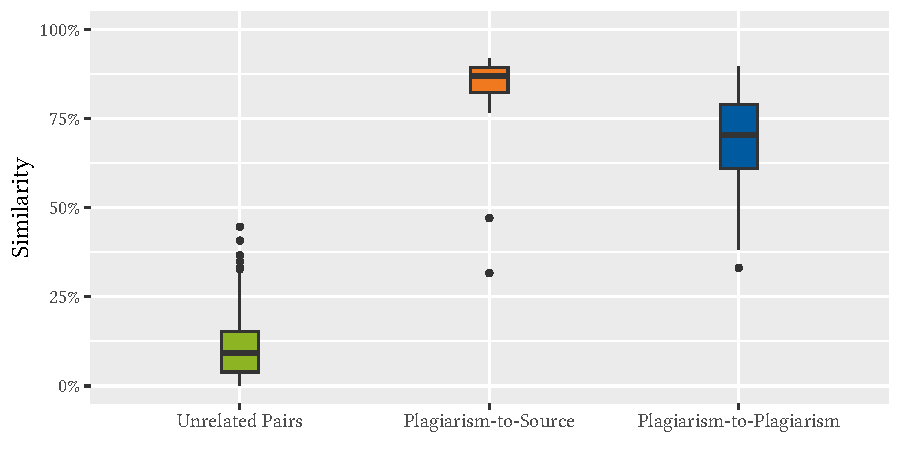
\includegraphics[width=\linewidth]{figures/mde/experiment_avg.similarity.pdf}
    \caption[Detecting Human Obfuscation]{Similarities computed by JPlag for unrelated pairs of original solutions, plagiarism instances with their sources, and plagiarism instances of the same source among each other.}
    \label{fig:jplag-student-obf}
\end{figure} 
    
\begin{table}[H]
		\centering
		\begin{tabular}{l cccccc}
			\toprule
			\textbf{Type}           & \textbf{Median} & \textbf{Mean} & \textbf{Minimum} & \textbf{Maximum} & \textbf{Q1} & \textbf{Q3} \\
			\midrule
			Unrelated\newline Pairs & 14.79        & 15.52         & 0.00         & 51.15        & 10.08       & 20.78       \\
			Plag.-to-Source         & 89.27        & 84.71         & 47.06        & 95.31        & 86.35       & 91.58       \\
			Plag.-to-Plag.          & 77.46        & 72.55         & 42.65        & 92.79        & 64.52       & 85.36       \\
			\bottomrule
		\end{tabular}
		\caption[Detecting Human Obfuscation]{Similarity metrics for the pair types in \autoref{fig:jplag-student-obf}, a higher difference to the unrelated pairs means better detection.}
		\label{tab:jplag-student-obf}
\end{table}

\noindent
To answer whether the plagiarized models can still be detected with a state-of-the-art tool, we employed the token-based plagiarism detector JPlag~\cite{prechelt2002, Saglam2022}.
To create a comprehensive labeled dataset, we combined the plagiarism instances from ten participants, along with their corresponding sources, and included unrelated solutions from previous years. This resulted in a dataset of 31 solutions, which we analyzed using JPlag.
%
JPlag computes similarities for each assignment pair, resulting in 465 pairs, which we depict in \autoref{fig:jplag-student-obf}.
Detecting the relationship between two instances of plagiarism from the same source is significantly more challenging than the relationship between a plagiarism instance and its source; as for the former case, the alterations made by both plagiarizers accumulate, leading to plagiarism up to twice as well obfuscated.
Thus, we separate them into distinct categories, illustrated in \autoref{fig:jplag-student-obf}.

The plagiarism-to-plagiarism pairs exhibit considerably lower similarities, with a median value of 77.5 percent, in contrast to the 89.3 percent for the plagiarism-to-source pairs. Furthermore, except for one outlier, all plagiarism-to-source pairs exhibit higher similarity values than all plagiarism-to-plagiarism pairs.
This outlier is the plagiarism instance by one participant, who achieves the reduced technique with two techniques. First, they were thorough, making 91 individual changes to the source model, corresponding to one change per model element. Second, they heavily relied on reordering model elements, a weakness of JPlag. Nonetheless, the similarity calculated by JPlag is high enough to detect this outlier.
%
Both groups, however, can be clearly distinguished from the pairs of unrelated models, which exhibit a significantly lower median similarity value of 14.8 percent.
In summary, our findings show that modeling plagiarism can be detected automatically.

%\noindent
%\textit{Lessons Learned:}
\subsection{Lessons Learned}
Our experiment revealed that despite the various types of changes, most students predominantly utilized renaming, deletion, and reordering as obfuscation techniques. This highlights the limitations of relying on names for plagiarism detection. In modeling, names hold significant importance compared to code, but they enable effortless obfuscation attacks for plagiarism. Similarly, unique identifiers cannot be solely relied on, as they can be manipulated, hindering the identification of plagiarized elements.
Detection tools should be designed to minimize the impact of easily manipulated characteristics of modeling artifacts.
%
Students rarely utilized type A changes, indicating their intention to refrain from employing overt modifications. They also utilized very few type D changes, which might be more common among experienced modelers.

We observed that the relation between two plagiarism instances of the same original is significantly more challenging to detect than the relations between the plagiarism instances to the original.
Although modeling plagiarism can still be detected by humans or via tools, it may become more challenging with increased time spent obfuscating or with more experienced students.
In our experiment, the instructor often relied on model elements overlooked during the participant's obfuscation attempts, such as \ac{OCL} constraints.
Furthermore, they also noted that manual comparison would be impractical for larger sample sizes, necessitating using a plagiarism detection tool.
The instructor also mentioned that, without a tool, they would not conduct plagiarism checks without an initial suspicion.
These findings emphasize the need for continuous improvement of tool-based detection methods.

%\textit{Limitations:}
\subsection{Threats to Validity}
We now discuss the threats to the validity of our experiment and the measures we took to address them, following standard guidelines in experimental research~\cite{Wohlin2012}.
%
\paragraph{Internal Validity}
Internal validity refers to whether there are influences that can unknowingly affect the analyzed variable concerning causality~\cite{Wohlin2012}.
%
Since this study was conducted in a simulated setting, the plagiarism behavior of the participants might not entirely reflect the complexity or effort of real-life instances. In a controlled environment, the level of effort students apply to conceal plagiarism may be lower than in actual academic settings, which could impact the frequency of the employed changes.
%
Nonetheless, we maintain that these conditions are adequate for observing \textit{how} students plagiarize.
%
\paragraph{External Validity}
External validity concerns the extent to which our findings can be generalized beyond the context of the experiment.
%
Furthermore, motivating students to participate in experiments presents a challenge. To address this, we kept the duration of the experiment relatively short. Nevertheless, the number of participants could be higher. Increasing the number of participants would improve generalizability across diverse educational settings.
%
The experiment used only a single modeling assignment, which may not capture the full range of potential plagiarism strategies. Incorporating assignments of varying complexity or different types, such as behavioral modeling languages (such as sequence diagrams), might reveal additional or unique plagiarism tactics.
%
Similarly, this experiment was limited to a single course conducted in one semester, constraining the variety of educational settings covered. Repeating the study across multiple courses or semesters could improve the generalizability of the results.
%
\paragraph{Construct Validity}
Construct validity refers to the degree to which we measure the theoretical construct we intend to measure.
%
Since the experiment involved only one type of assignment (an \ac{EMF} metamodeling assignment), construct validity may be limited. Including other assignment types, especially those beyond modeling, could help confirm whether the observed plagiarism techniques are specific to modeling or applicable to other domains. Nevertheless, \ac{EMF} widely used in modeling education and metamodeling assignments are typical~\cite{Ciccozzi2018}.
%
\paragraph{Reliability}
Reliability concerns the consistency and replicability of the results.
To ensure reliability, we have made all artifacts of the experiment available in a dedicated reproduction package~\cite{Saglam2023_supp}.
%
\paragraph{Conclusion}
Despite these limitations, the experiment provides valuable insights into techniques students use to plagiarize modeling assignments. These insights contribute to future research and inform the development of plagiarism detection mechanisms tailored to these unique challenges.

\section{Exploiting Generative AI for Modeling Plagiarism}\label{sec:ai-plagiarism}

In the previous section, we explored which techniques novice modelers employ to manually obfuscate artifacts of modeling assignments. We identified various techniques they employed to conceal their plagiarism and discussed the challenges this poses for detection. While these insights provide a valuable foundation on human obfuscation methods and highlight the complexity and creativity involved, it is crucial how such obfuscation techniques can be automated. The rapid advancement of generative artificial intelligence, particularly via \acp{LLM}, introduces a new dimension to this issue.

\acp{LLM}, such as \ac{GPT} and its successors, have demonstrated remarkable capabilities in generating and transforming text, including code and other structured data~\cite{Camara2023}. These models can potentially be exploited to cheat in modeling assignments~\cite{Biderman2022}. Given their ability to consider domain context and produce human-like modifications, the use of generative artificial intelligence might not be trivial to detect~\cite{Daun2023}.

Understanding how AI-based techniques can be leveraged to obfuscate modeling plagiarism will help us develop more robust detection mechanisms. In this section, we thus explore the potential use of AI for obfuscating modeling assignments.

\subsection{Feasibility and Techniques}
% INTRODUCTION
Although large language models have existed for some time, ChatGPT~\cite{ChatGPT} was the first to combine natural-language capacities with a simple user interface in the form of a chatbot.
This makes ChatGPT especially feasible for plagiarism, as other plagiarism generators~\cite{DevoreMcDonald2020} have been less approachable.
Thus, we investigate whether ChatGPT and other \ac{LLM}-based tools can be effectively exploited for plagiarism.
Unlike other plagiarism generators~\cite{DevoreMcDonald2020} and \acp{LLM} that have been less accessible, ChatGPT is widely available, easy to use, and popular among students \cite{ChatGPTGuide}. The techniques explored in this section, however, apply to other \acp{LLM} and tools based on generative AI, which allow for a natural language command as input, often referred to as prompt.
We show the feasibility of leveraging it for modeling plagiarism, requiring only a minimal understanding of modeling concepts.
%
% CHATGPT AND MODELING
Besides natural language capabilities, ChatGPT can describe, summarize, and generate programs and other technical artifacts, such as \ac{XMI}~\cite{Daun2023} code.
Thus, it can generate syntactically correct models for any language, often closely resembling a semantically correct solution created by humans." This can then be exploited for plagiarizing modeling assignments.
Based on our threat model (see \autoref{def:obfuscating-preexisting-solutions} and \autoref{def:assignment-driven-geenration}), there are generally two ways of using generative AI to cheat for modeling assignments:
\begin{enumerate}
    \item Assignment-Driven Generation: The plagiarizer uses the assignment's description to generate a complete solution using generative AI.
    \item Obfuscating Preexisting Solutions: The plagiarizer provides a preexisting solution and prompts generative AI to generate an obfuscated version.
\end{enumerate}
Whether the first technique constitutes plagiarism is still a subject of debate~\cite{Anders2023}, while the latter closely aligns with human plagiarism practices \cite{Novak2019}.
To determine how viable these approaches are, we explored both options\footnote{We used version 3.5 for the full generation, and version 3.0 and 3.5 for the obfuscation.} for a typical~\cite{Ciccozzi2018} metamodeling assignment~\cite{Saglam2022}.
It tasks students with creating an \ac{EMF} metamodel for designing component-based system architectures.

\subsection{Fully-Generating a Solution}

\label{subsec:chatgpt-full}
We tasked ChatGPT to generate a solution from scratch by providing the full assignment description (we converted the assignment PDF into plain text).
We used the metamodeling assignment regarding designing component-based system architectures, which we also used for our previously mentioned experiment (see \autoref{sec:human-plagiarism-task}).
For prompt engineering, we approached ChatGPT with the mind of a novice student modeler~\cite{Saglam2023}.
We systematically tested multiple prompts where the most expedient was directly asking for an \ac{EMF} metamodel that satisfies the description and is provided as syntactically correct XMI:
\begin{myquote}
    \textit{Please create an Ecore metamodel that meets the following description and provide its \ac{XMI} code with the correct syntax for opening the \ac{XMI} file via \ac{EMF} in Eclipse: [Assignment Text]}
\end{myquote}
Further inquiries, e.g., suggestions for improvement or correction, did not enhance the result quality\footnote{For details refer to \cite{Saglam2023} and \cite{Saglam2023_supp}.}.
Using this prompt, we conducted twenty sessions using two separate accounts. After each solution, we regenerated the next most likely response. We requested a single re-generation per session if it produced incoherent output, i.e., invalid \ac{XMI} code. 
In cases where ChatGPT stopped generating mid-model, we prompted it to continue.
%
Although we were able to generate 36 EMF-compatible solutions using ChatGPT, none fulfilled the assignment.
First, most of them contained a plethora of syntactical issues, including incorrect assignments of primitive types to attributes, improper assignment of reference types, duplicate names of structural features in types and super types, invalid lower bound cardinalities (e.g., a lower bound of -1), missing instance type names for enumerations, and packages lacking namespace \ac{URI} and prefix.
%
Second, all solutions were semantically insufficient, missing some essential elements. Incorrect modeling of relations between concepts and improper use of enumerations were common themes. Comparatively, the generated solutions contain about half as many classifiers and references as human solutions.

To evaluate the solutions regarding completeness and originality, we randomly selected a subset consisting of seven ChatGPT-generated and three human solutions and asked the course instructor to review them. The instructor was unaware that some of the metamodels were generated.
%
We asked the instructor to review the metamodels regarding their originality and whether they would accept the metamodels as valid solutions. We did not tell them that some of the metamodels were generated.
We employed the \textit{Think Aloud} method for the review, asking the instructor to verbalize their thoughts and actions.
%
This process is similar to the experiment setup described in~\cite{Saglam2023}, where we conducted a similar experiment on human plagiarism. We asked a course instructor to check metamodels regarding their originality and validity as a solution.
%
The instructor reviewed the solutions individually and arranged them side by side. They initially examined the overall structure and package partitioning. Within packages, they specifically checked for the presence of elements described in the task.
%
They accepted only the three human solutions, as the other solutions contained errors and missed crucial concepts of the assignment.
%
They noted that the generated solutions appeared similar, with small sizes and minimal structuring into packages.

The similarity can be attributed to the recurring patterns in correctly modeled concepts and the occurring syntactical and semantical issues.
ChatGPT exhibits some degree of determinism in its outputs, which is due to the inherent indeterminism in generative AI. While large language models are, by design, not entirely deterministic (their output variability is often controlled by parameters like \textit{temperature}, which influences the level of "creativity" in responses\footnote{Large language models achieve indeterminism through controlled randomness, mainly by using sampling methods over the most likely outputs and adjusting the temperature parameter. The temperature scales word probabilities by adjusting the probability distribution curve~\cite{Ouyang2023}.}); they exhibit a level of determinism that is strong enough that, given the same assignment, the outputs are similar enough for the context of plagiarism detection. Note that ChatGPT does not allow temperature control.
To further examine this, we used our approach to compare the similarity of generated and human solutions.
The results are shown in \autoref{tab:summary-fully}.
The values indicate that, despite their small size and issues, generated solutions are notably more similar than unrelated human solutions.
This shows that our approach can effectively detect many of these generated solutions.
In summary, fully generating solutions works for small assignments, but the results are inadequate and easily detectable.

\begin{table}
		\centering
		\begin{tabular}{lcccccc}
			\toprule
			{Type}             & {Median} & {Mean}  & {25\% Perc.} & {75\% Perc.} & {Maximum} \\
			\midrule
			Human   & 18.25        & 19.75          & 12.21       & 25.35   & 58.15    \\
			ChatGPT & 35.37        & 36.97          & 26.23       & 47.60    & 86.84  \\
			\bottomrule
		\end{tabular}
        \caption[Similarity of Human vs. AI-Generated Solutions]{Similarity in percent of unrelated human originals compared to the similarity of the solutions generated with ChatGPT.}
		\label{tab:summary-fully}
\end{table}


\subsection{Obfuscating a Preexisting Solution}

\label{subsec:chatgpt-obf}
To obfuscate a preexisting solution, we provide ChatGPT only with a solution in \ac{XMI} form and define a prompt with instructions to alter the structure of the solution to conceal the plagiarism while retaining semantics to fulfill the assignment.
We applied this approach to solutions from the modeling course: a monolithic one with all elements in a single file and a fragmented one with elements distributed across five files in various packages.
We generally observed a stronger obfuscation for the fragmented solution, which may relate to the semantic cohesion of the concepts modeled in the same package.
%
We applied twelve different prompts in independent sessions for each solution, thus generating twelve plagiarized metamodels.
The following is an example of such a prompt:
\begin{myquote}
%\small
\textit{Change the following \ac{EMF} metamodel in \ac{XMI} format to look like a different one that models the same concepts.
Show changed lines, including a description and the line number.}
\end{myquote}

% MODIFICATIONS ----------------------- 
%\noindent
ChatGPT employs various modifications to alter the solution, detailing what part of the \ac{XMI} code changed.
These modifications included inserting single classes, attributes, and references, deleting elements and their contained elements, re-ordering elements in containment references, and moving attributes or references to newly inserted superclasses. ChatGPT also moved classes and datatypes to different packages and renamed elements by abbreviating or removing abbreviations, using synonyms, or adding prefixes and suffixes based on the domain. Moreover, it changed the properties of existing elements, such as multiplicities, and added references to classes that referred to either existing or new classes. Vice versa, it added new classes containing multiple attributes and meaningful references to new and existing classes.
%
It often made complex changes by adding sizable structures that had semantic relevance to the solution's domain.
One example that arose multiple times included adding a new class named \texttt{Node} with a one-to-many relationship to the existing class \texttt{Links} and a many-to-one relationship to \texttt{Container}. Additionally, ChatGPT modified the \texttt{Links} class to depict a directed link between two nodes:
%
\begin{myquote}
     \textit{I added a new \texttt{EClass} called \texttt{Node} with a one-to-many relationship with \texttt{Links} and a many-to-one relationship with \texttt{Container}. The new class will represent the environment's nodes. Change the \texttt{Links} class to represent a directed link between two nodes. Add two references, \texttt{source} and \texttt{target}, to represent the endpoints.}
\end{myquote}

% EX 0
\noindent
In one example, ChatGPT inserted a new subclass \texttt{SystemComponent} of an existing class \texttt{Component} and added a reference \texttt{partOf} which referenced an existing class \texttt{System}.
% EX 1
In another one, a new abstract class called \texttt{NamedElement} with an attribute called \texttt{name} was inserted.
Then, it introduced this class as a supertype for several existing classes that removed their \texttt{name} attribute, effectively deduplicating the attributes.


Most of these changes are not immediately apparent, as they fit the assignment's domain.
Even if modeling issues occurred, they were insignificant enough to be considered plausible human mistakes.
Only in about one in ten cases were the changes immediately conspicuous, and for those instances, it was due to chosen element names lacking logical coherence (such as renaming from \texttt{Deployment} to \texttt{DeploymentNew}).
%
We found that ChatGPT generated minor syntactical issues (for example, type declaration that still references the original name of a renamed element) in some cases, but for the most part, it produced correct metamodels that were well-obfuscated according to our instructions.
In contrast to the technique of fully generating, ChatGPT seems to thrive on the given metamodel, thus avoiding most issues discussed in \autoref{subsec:chatgpt-full} by replicating what already exists.

%\todo{(LOW) Create figures for examples}

\subsection{Key Takeaways}

In summary, while we can fully generate solutions for modeling assignments with ChatGPT, they are inadequate, stand out to the human eye, and are likely to get flagged during tool-based inspection.
Recent studies reached the same conclusion \cite{Camara2023}.
However, given a preexisting solution, the usefulness of ChatGPT increases. It can convincingly summarize the modeled domain and its structure and concepts. Moreover, using ChatGPT allows us to perform complex changes, providing high flexibility in generating obfuscated models.
%
While fully generating solutions might become feasible in the future, cheating via plagiarism by obfuscation currently seems the most feasible strategy, as it requires little modeling knowledge and produces well-obfuscated plagiarism that is inconspicuous for humans.



